\chapter{Literature review}
This chapter provides an overview of past research done regarding the control of hexapod movement and sensing methods. First a brief history of hexapods is presented after which various terrain sensing and adaptation methods are presented.

\section{Hexapod history}
Hexapoda, Greek for "six legs" refers the group of arthropods possessing three pairs of legs. As an example see a flesh-fly in \autoref{fig:flesh-fly}.

\begin{figure}[h]
    \centering
    \begin{minipage}{.5\textwidth}
        \centering
        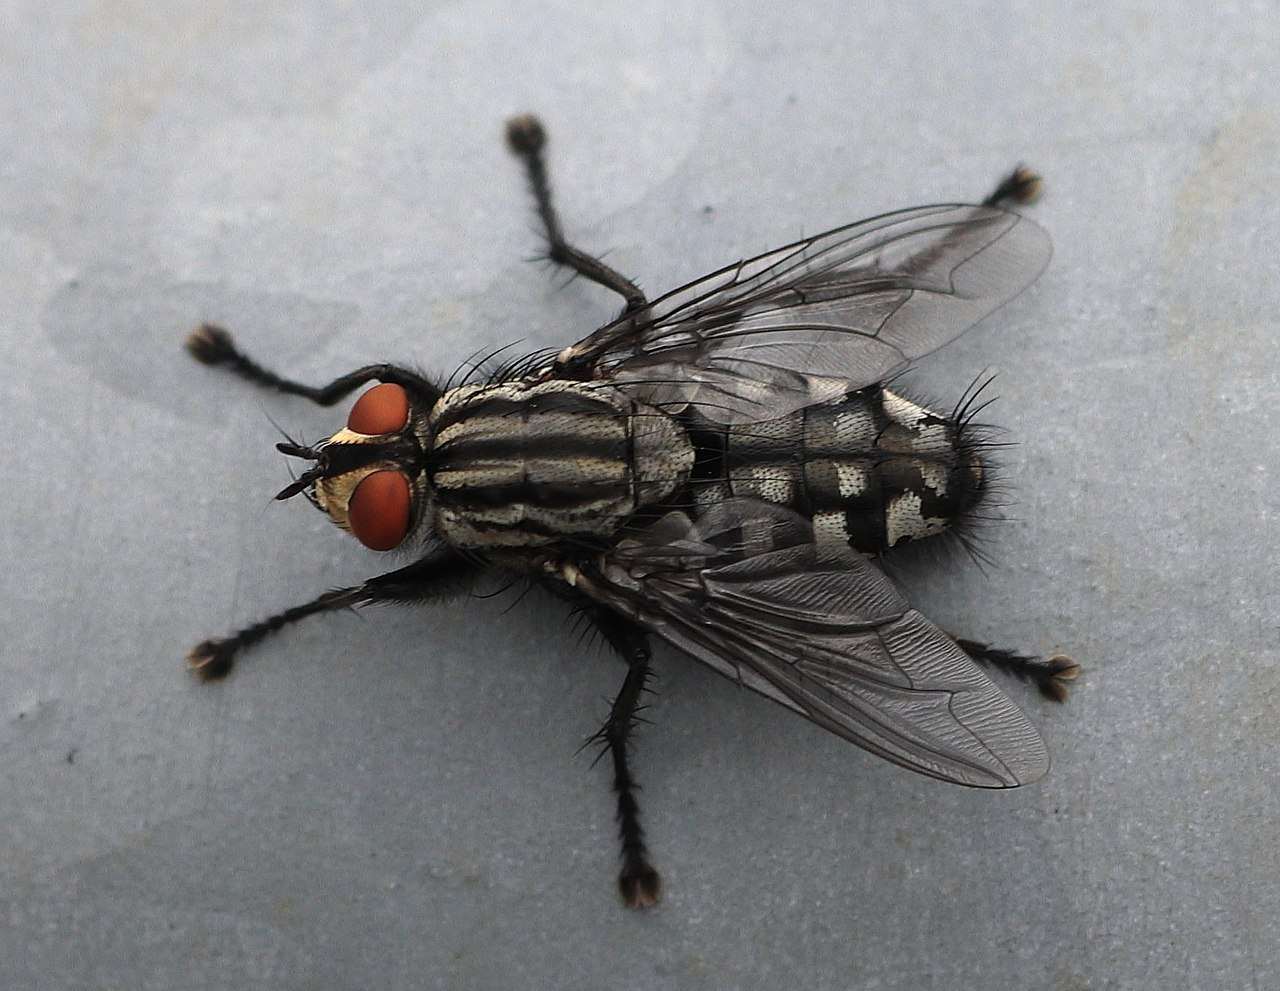
\includegraphics[height=4cm]{flesh-fly.jpg}
        \caption{A Flesh-fly}
        \label{fig:flesh-fly}
    \end{minipage}%
    \begin{minipage}{.5\textwidth}
        \centering
        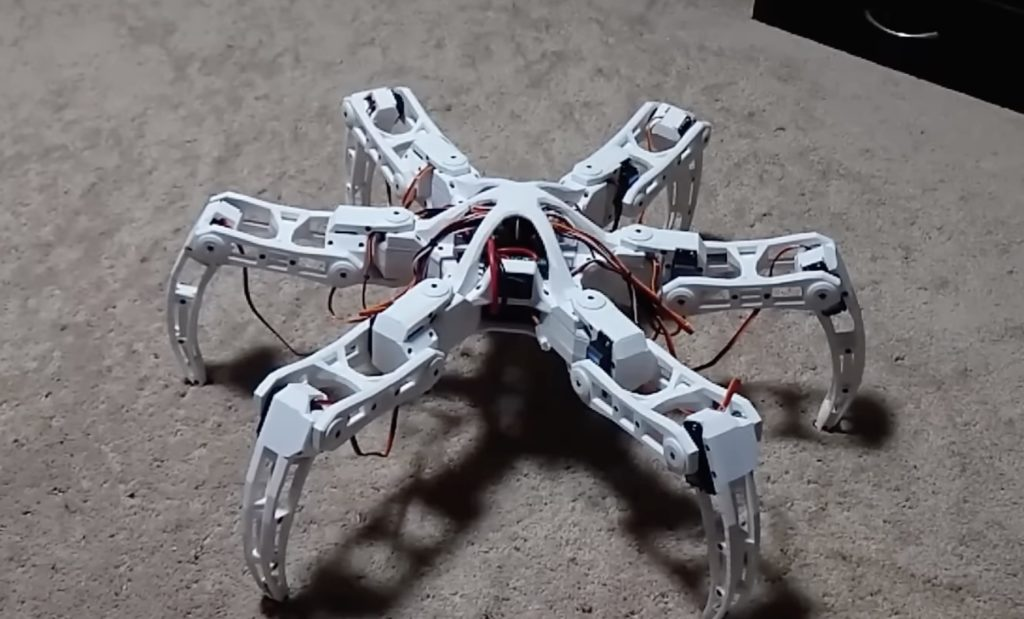
\includegraphics[height=4cm]{circ-hexapod.jpg}
        \caption{A circular hexapod}
        \label{fig:circ-hexapod}  
    \end{minipage}
\end{figure}

In the context of robotics "Hexapod" is used to refer to any robot with six legs, the most common configuration of Hexapods are either a rectangular
layout with three legs on either side mimicking biological Hexapoda, or a circular design with radially symmetrical leg spacing, as seen in \autoref{fig:circ-hexapod}

The hexapod possess the minimum number of legs to allow a naturally stable platform since while taking a step there can be upwards of three anchor points around the center of mass at all times. This makes the hexapod hexapods an ideal platform to navigate complex terrain while maintain stability, without requiring advanced balancing control systems.

For a hexapod to walk it must lift some of its legs while bracing with others, the number of swinging to bracing legs, and how each is moved, is referred to as the walking "gait". The chosen gait influences the speed and stability of the hexapod, the tripod gait is considered to be the most well rounded, having good speed and stability. In the tripod gait three legs are bracing while the remaining three swing. A example of a more stable gait would be the One by One gait, where only one leg is moved at a time.

It is also possible to create a system where there is no predetermined gait, but rather the system determines the optimal legs to brace and swing depending on the current walking environment.

\section{Control}
Walking over rough terrain requires a control system to correctly actuate the hexapods legs. Various types of control schemes exist, the primary schemes are traditional controllers, bio-inspired controllers and \ac{rl}. These three schemes are discussed below. Control trends can be seen in \autoref{fig:control-trends}
\begin{figure}[h]
    \centering
    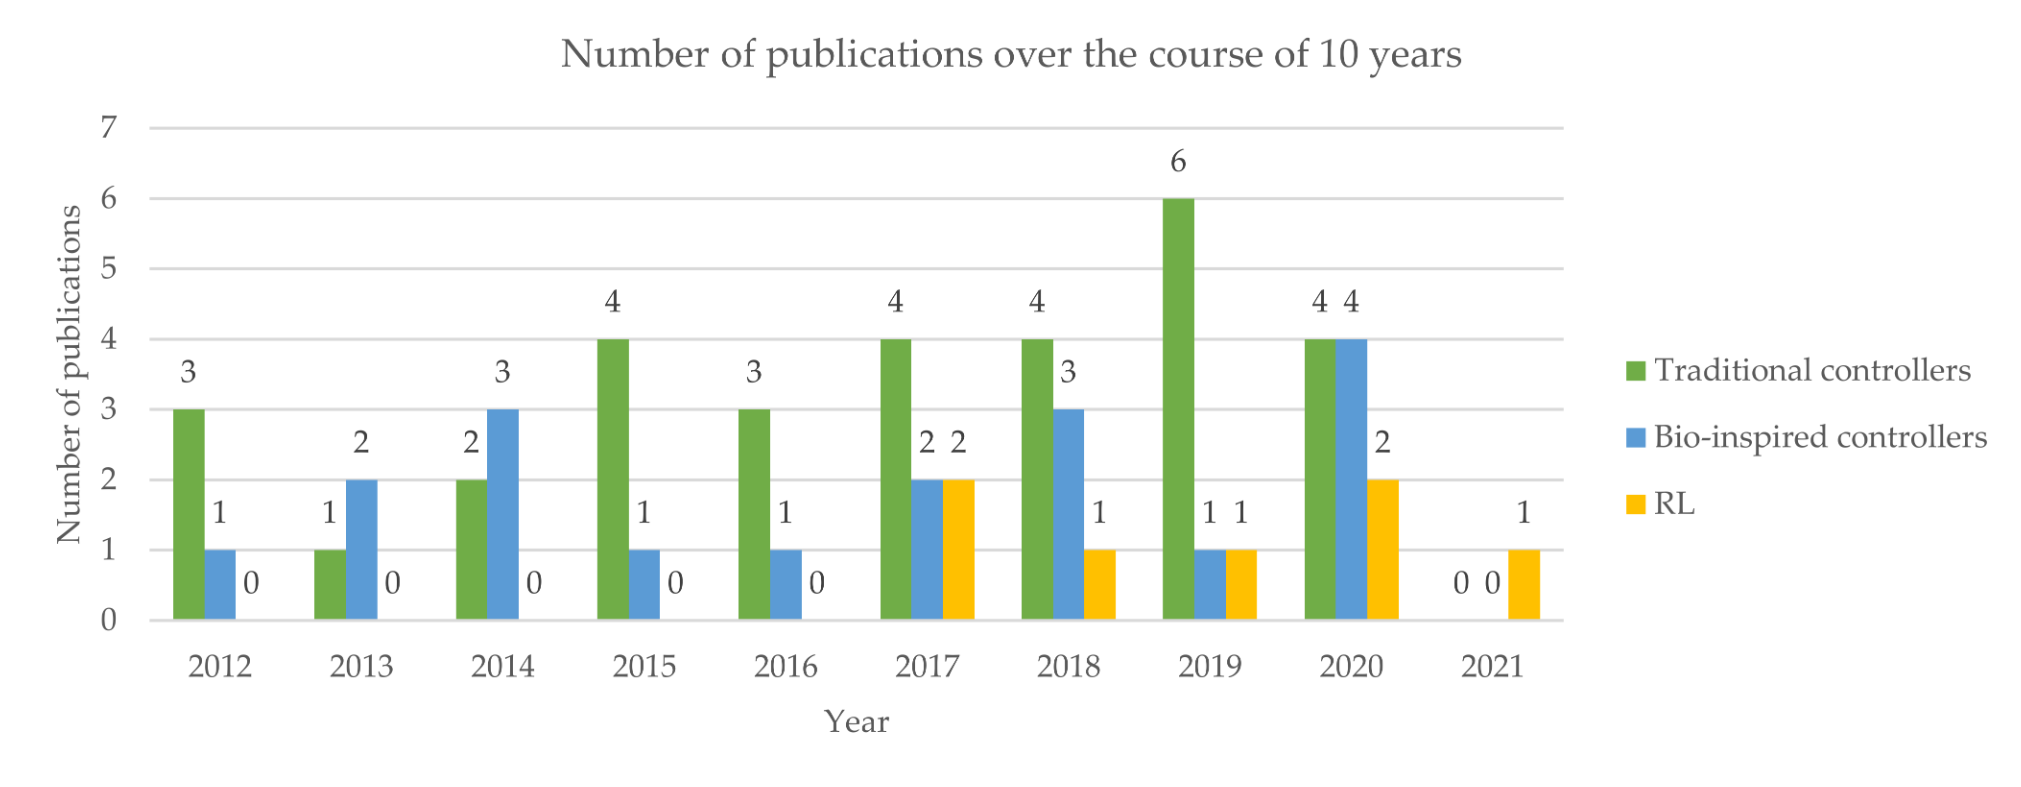
\includegraphics[width=\textwidth]{contoroller-trends.png}
    \caption{Trends of hexapod control schemes \citep{coelho2021trends}}
    \label{fig:control-trends}
\end{figure}

    \subsection{Traditional}
    Traditional controllers rely on an exact mathematical model of the robot and \ac{ik} to calculate angular commands for all leg joints. This method of control is purely kinematic does not take into account external forces applied to the robot, thus it does not inherently adjust to the environment.

    Instead of a purley kinematic model, a dynamic model can also be used. Using a dynamic model the forces acting on the robots legs are taken into account usually acquired through torque measurements from servos. By taking applied torque into account dynamic model controllers will intrinsically detect a deviation when an external force is applied to the robot or its legs and compensate appropriately.

    It should be noted that it is possible for a kinematic model controller to also adjust to external disturbances, but this is not intrinsic to the control model and requires additional control logic.
    
    \subsection{Bio Inspired}
    Bio inspired controllers attempt to mimic the neural structure of animals to achieve the same locomotion methods that they use. This is implemented through the use of a \ac{ann} If implemented successfully a bio inspired controller can be highly adaptable to the surrounding environment and is even able to adapt to damaged or missing legs.

    \subsection{\acl{rl}}
    \ac{rl} controllers are created through using trial and error to construct a neural net that minimises a cost function for a specific goal. This theoretically allows \ac{rl} controllers to adapt to any circumstances given enough time, allowing a very hight level of autonomy, as no prior direction is required. \ac{rl} controllers are though notoriously difficult to train properly, especially when the amount of sensors and control outputs grow large, increasing the feature space. And event he most well trained \ac{rl} agent still has the possibility to exhibit inexplicable behaviour.
    
\section{Sensing Methods}
    No matter the control scheme used, to know where to place its feet the robot requires sensor(s) to sense its environment in some way,
    this could be achieved through simple sensors such as servo torque or touch. More advanced methods such as vision or \ac{lidar} are also used.
    \cite{homberger2017terrain} uses stereoscopic vision to adjust end effector height and to classify surface materials.

    Depending on the terrain navigation system it might be required to localise the robot in 3D space, for this it is possible to use external sensors such as a type of beacon (RF, Reflective, Ultrasonic), \ac{gps} or, through the use of a \ac{slam} system, internal sensors such as vision could be used.

    % \subsection{End Effector Placement Method}

    % Among other research focused on hexapods, many focus on topics such as obstacle avoidance, climbing surfaces, confined surfaces and cargo transportation.
    % When focusing of terrain adaptation most often the use of sensors such as \ac{lidar}, torque, or touch are employed. Where usually the height of end effectors
    % are adjusted to the height of the terrain \cite{coelho2021trends}.

    % Some papers, such as \cite{homberger2017terrain} utilise stereoscopic vision, in addition to end effector height adjustment, also focus on surface material classifications based on which the virtual stiffness of the impedance controller is adjusted.

    % The focus of this paper will be on end effector height and planar position adaptation through real time walkability classification of the environment. 
    % While only utilising an \ac{rgbd} camera as sensor

    % \subsection{Localisation and Mapping}

    % This project requires a system that will localise the robot within its environment, as the primary sensor used is an \ac{rgbd} camera various visual \ac{slam} systems were considered. ORB-SLAM 3, a optimisation-based, sparse map \ac{slam} system was chosen to be used. ORB-SLAM 3 maintains a sparse map, an atlas, of both active and dormant features. This atlas is used to localise in the sparse map \citep{macario2022comprehensive}.

    % The implementation of a dense map to be used for end effector placement is discussed in \autoref{chap:mapping}.

\section{Simulation Environment}

The most popular physics simulators for robotics in recent times are Gazebo, \ac{mujoco} and CoppeliaSim (previously V-REP) \citep{Collins-2021}.
Gazebo and CoppeliaSim both have easy to use \ac{gui} interfaces and easy integration with \ac{ros}. \ac{mujoco} on the other hand does not have
a full \ac{gui} interface, only a simulation viewer, and does not have native \ac{ros} integration. Having said this \ac{mujoco} was found to be
the most accurate and fastest simulator when considering the use case of robotics \citep{Erez-2015}.

\section{Uneven Terrain}
    As hexapods are inherently stable, they are good candidates for use in uneven terrain, and this tends to be where much hexapod research is focused.
    Such as in \cite{homberger2017terrain}, which uses a stereoscopic camera to extract features and classify terrain by factors such as material type,
    slope and granularity. These parameters are then used to classify various gait parameters, such as step height and dampening, to improve stability while
    walking.

    This is similar to \cite{Xu2023Learning}, which aims to
    classify terrain based on material properties, however, \cite{Xu2023Learning} focuses on characterising terrain through touch sensors instead of visual sensors.
    This is achieved through the use of machine learning.
    
    Moving away from gait optimisations and local terrain classification, \cite{Prágr2019Online} aims to characterize
    large areas of terrain in terms of navigational efficiency through the use of gaussian processes and a incrementally constructed spatial map.
    An example of this exploratory traversability classification can be seen in figure \ref{fig:cite_pragr}.
    \begin{figure}[h]
        \centering
        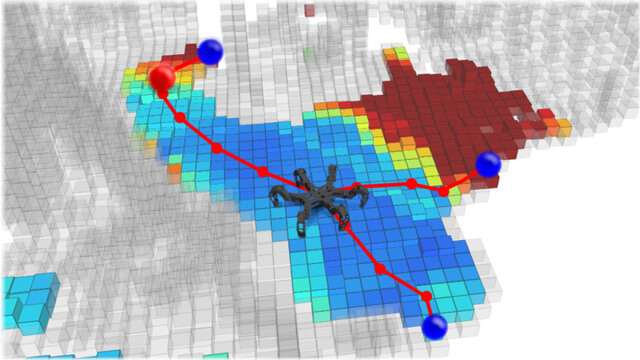
\includegraphics[width=0.7\textwidth]{cite_Pragr.jpg}
        \caption{Exploratory terrain traversability classification from \cite{Prágr2019Online}}
        \label{fig:cite_pragr}
    \end{figure}

    \newpage
    \noindent
    While this paper is on hexapods, it should be noted that much work has also been done on quadrupeds. For example \cite{Mastalli2020Motion} uses various sensors
    to assign a cost to surrounding terrain, thus constructing a cost map, this cost map is then used to select optimal foot end positions for the next step. This can be seen in
    figure \ref{fig:cite_quadruped_walk}.
    \begin{figure}[h]
        \centering
        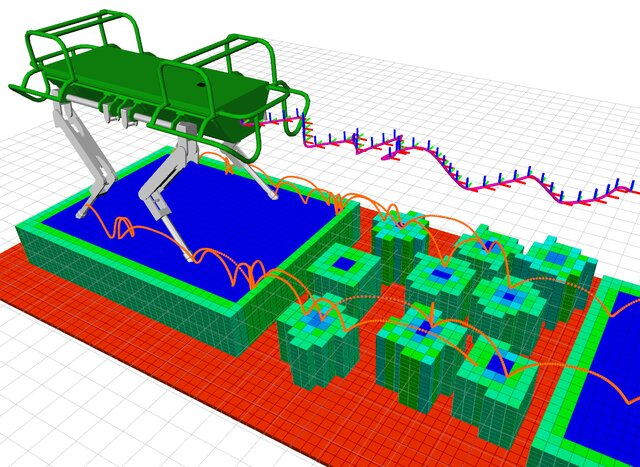
\includegraphics[width=0.8\textwidth]{cite_quadruped_score_map.jpg}
        \caption{Quadruped terrain scoring and navigation from \cite{Mastalli2020Motion}}
        \label{fig:cite_quadruped_walk}
    \end{figure}
    Of course, being a quadruped, in addition to finding optimal foot end positions, significant consideration had to be given to maintaining the stability of the robot,
    something that is much less of a concern with hexapods.

\section{Research Decisions}
    This research paper focuses on using vision based mapping, terrain classification and the optimisation of foot end positions, thus it was decided that
    traditional kinematic control is used as it is the simplest and most predictable method of control. Thus allowing the focus to remain on terrain
    classification and foot end position optimisation.

    The camera that is used is the Intel Realsense D435i \ac{rgbd} camera, incorporating stereoscopic cameras and a \ac{lidar} sensor.
    This camera also has a extensive existing codebase and support that ensures accurate depth readings are attained.

    A system to localise the robot within its environment is required, as the primary sensor used is an \ac{rgbd} camera, various visual
    \ac{slam} systems were considered. ORB-SLAM 3, a optimisation-based, sparse map \ac{slam} system was chosen to be used. ORB-SLAM 3 maintains
    a sparse map, an atlas, of both active and dormant features. This atlas is used to localise in the sparse map \citep{macario2022comprehensive}.
    The implementation of a dense map to be used for end effector placement is discussed in \autoref{chap:mapping}.
    \textcolor{red}{Compare this more to others?}

    Finally a simulation environment was chosen. \ac{mujoco} has exceptional contact physics simulation and the only relevant
    downside is the lack of native \ac{ros} integration and the lack of a comprehensive \ac{gui}, which seeing as \ac{mujoco} has good python bindings,
    could be seen as a advantage. Considering this, \ac{mujoco} was chosen as the simulator.


\bigskip
\bigskip
\hrule
\smallbreak
\hrule